\documentclass[12pt,titlepage]{article}

\setlength{\oddsidemargin}{0in}
\setlength{\evensidemargin}{0in}
\setlength{\textwidth}{6.5in}
%
\setlength{\textheight}{9in}
\setlength{\topmargin}{0in}
\setlength{\headsep}{0in}
\setlength{\topskip}{0in}
\setlength{\headheight}{0in}

\usepackage{graphicx}
\usepackage{times}
\usepackage[plainpages=false, colorlinks=true, anchorcolor=blue, linkcolor=blue, citecolor=blue, bookmarks=false, urlcolor=blue]
{hyperref}
\usepackage[square,comma,authoryear]{natbib}


\title{DOE Office of Science INCITE Project:\\
{\it Extreme-scale Simulation of Supernovae and Magnetars from Realistic Progenitors}\\
2019 Q1 Report}

\author{Principal Investigator:\\Sean M. Couch\\
  Michigan State University \vspace{0.1in}\\
  Co-Investigators: \\
  Andrew Christlieb (Michigan State University) \\
  Evan O'Connor (Stockholm University)\\
  Kuo-Chuan Pan (National Tsinghua University) \\
  Luke Roberts (Michigan State University) \\
  MacKenzie Warren (Michigan State University) \\
}

\date{April 1, 2019}


\begin{document}


\maketitle


%%%%%%%%%%%%%%%%%%%%%%%%%%%%%%%%%
\section{Project Usage}

%%%%%%%%%%%%%%%%%%%


% \begin{figure}
%   \begin{tabular}{cc}
%     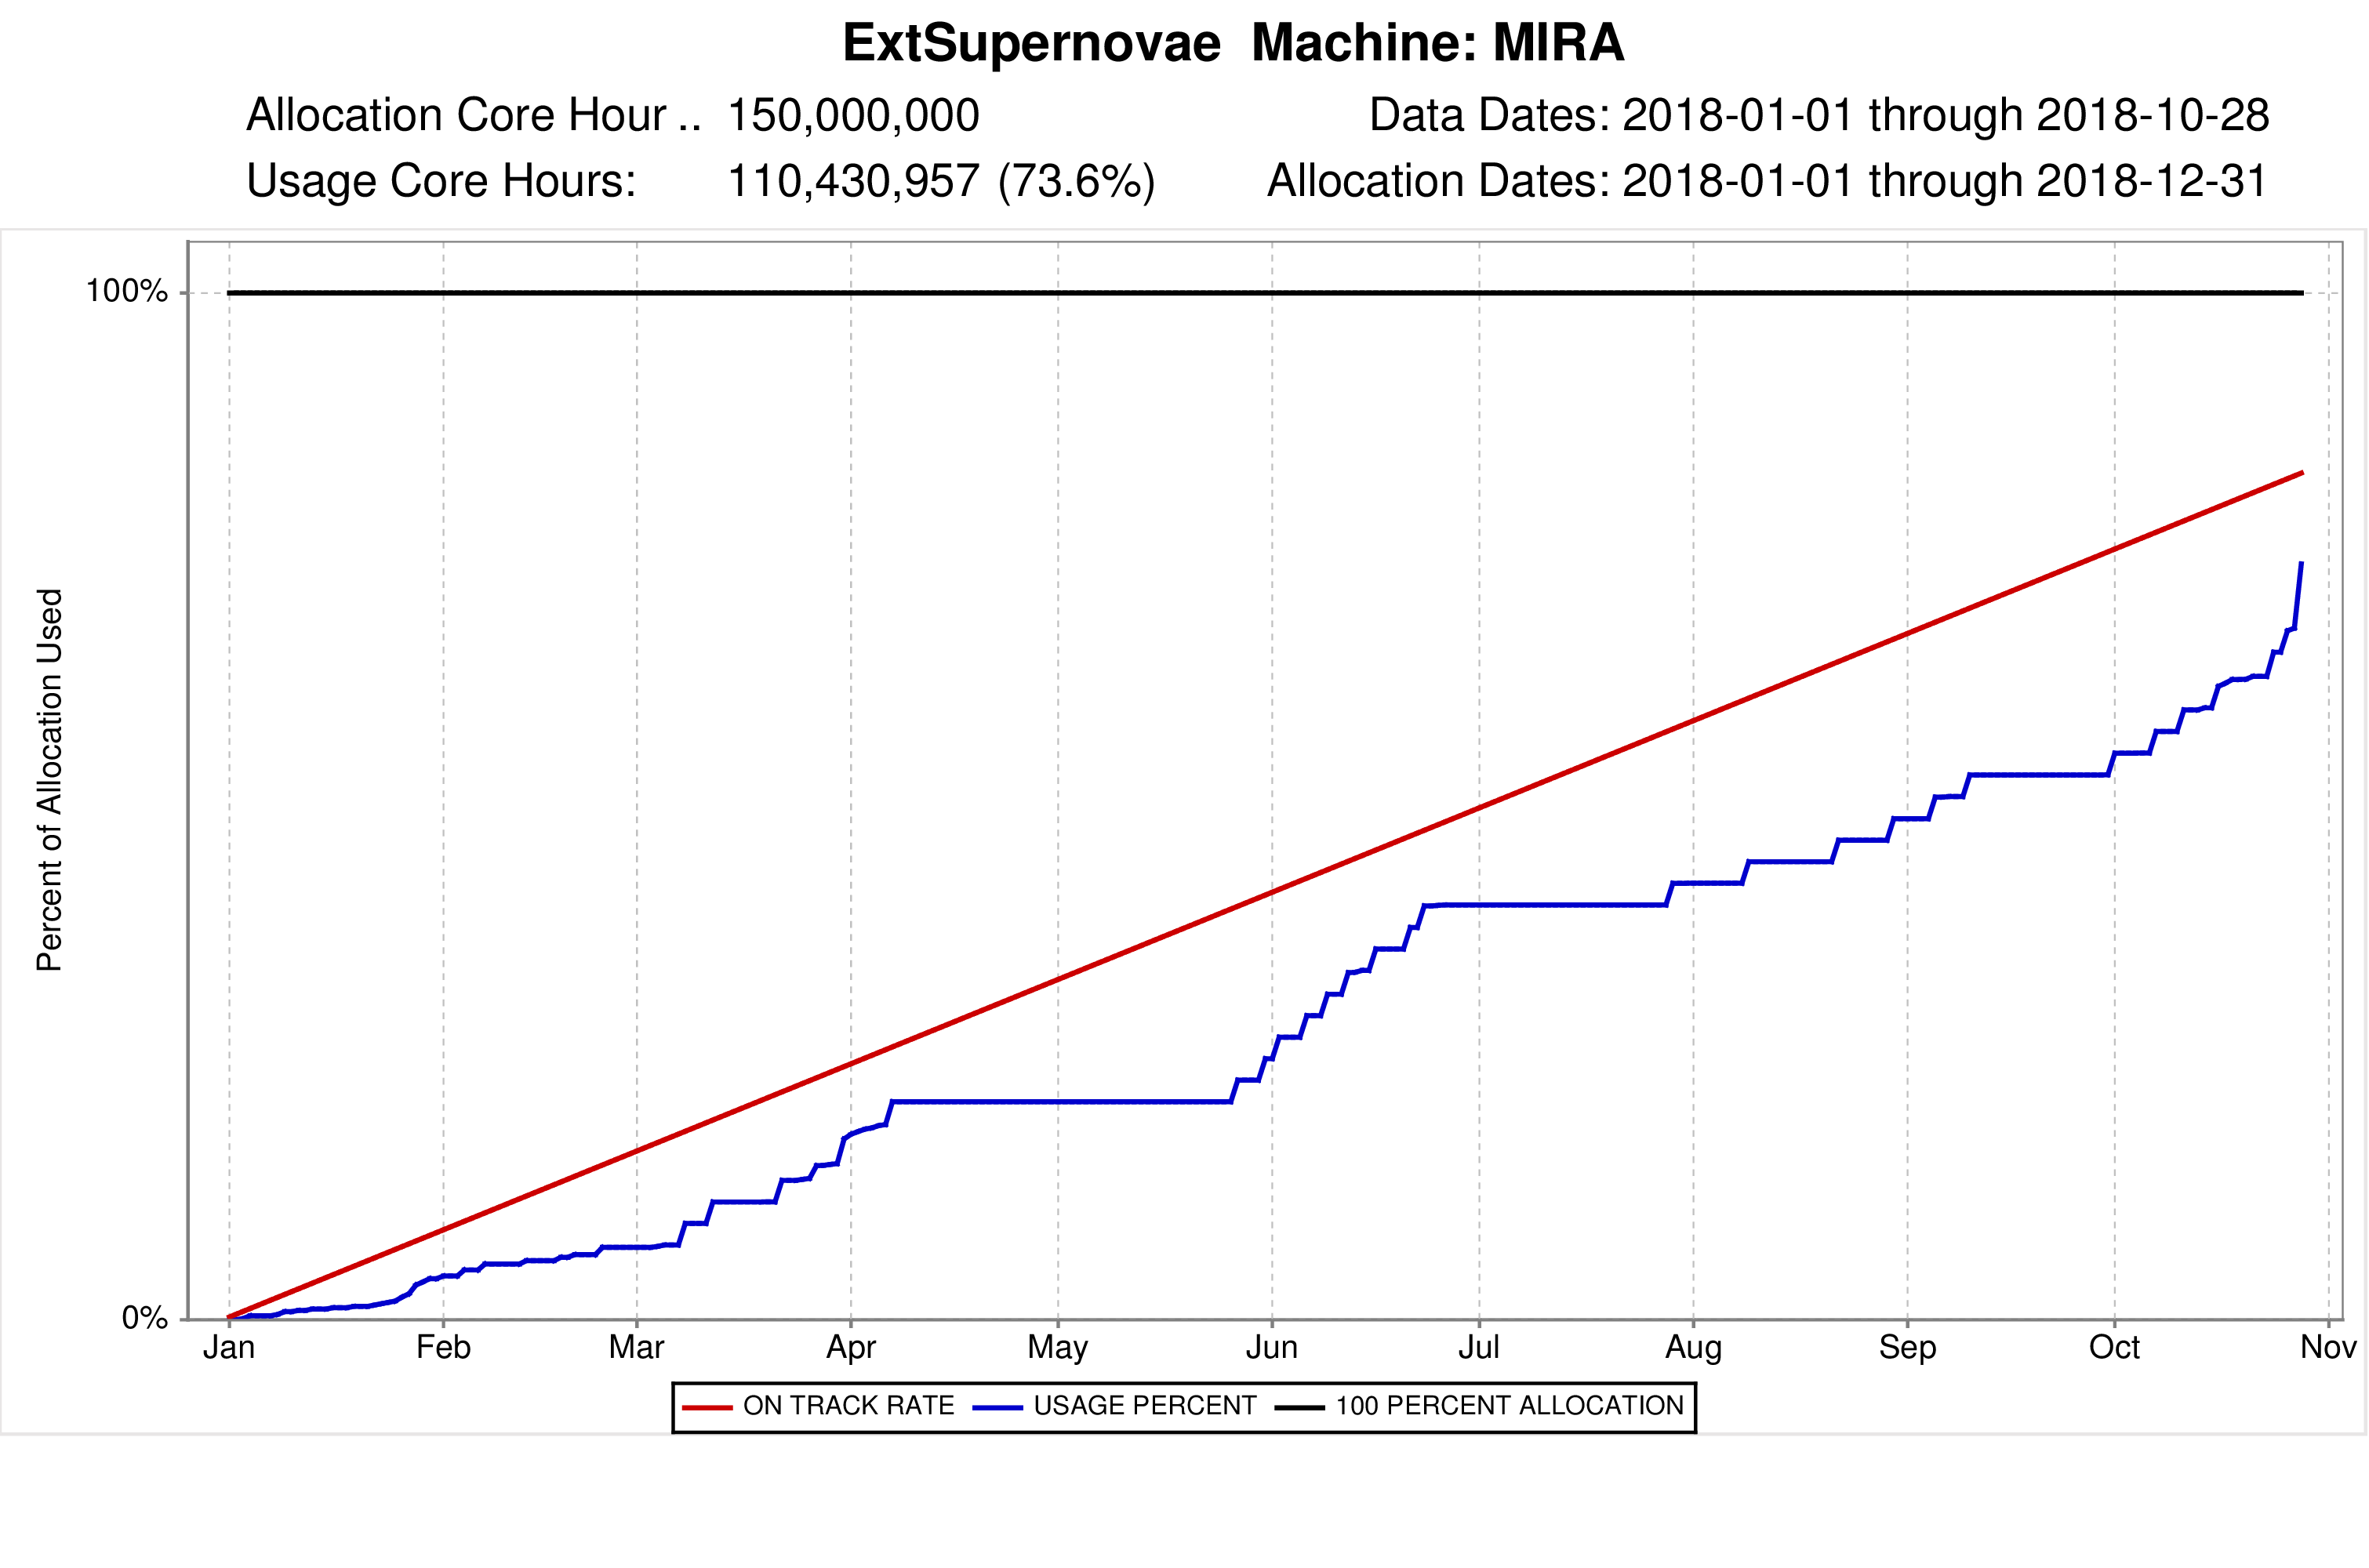
\includegraphics[width=3.25in]{on_track_graph_mira.png}
%     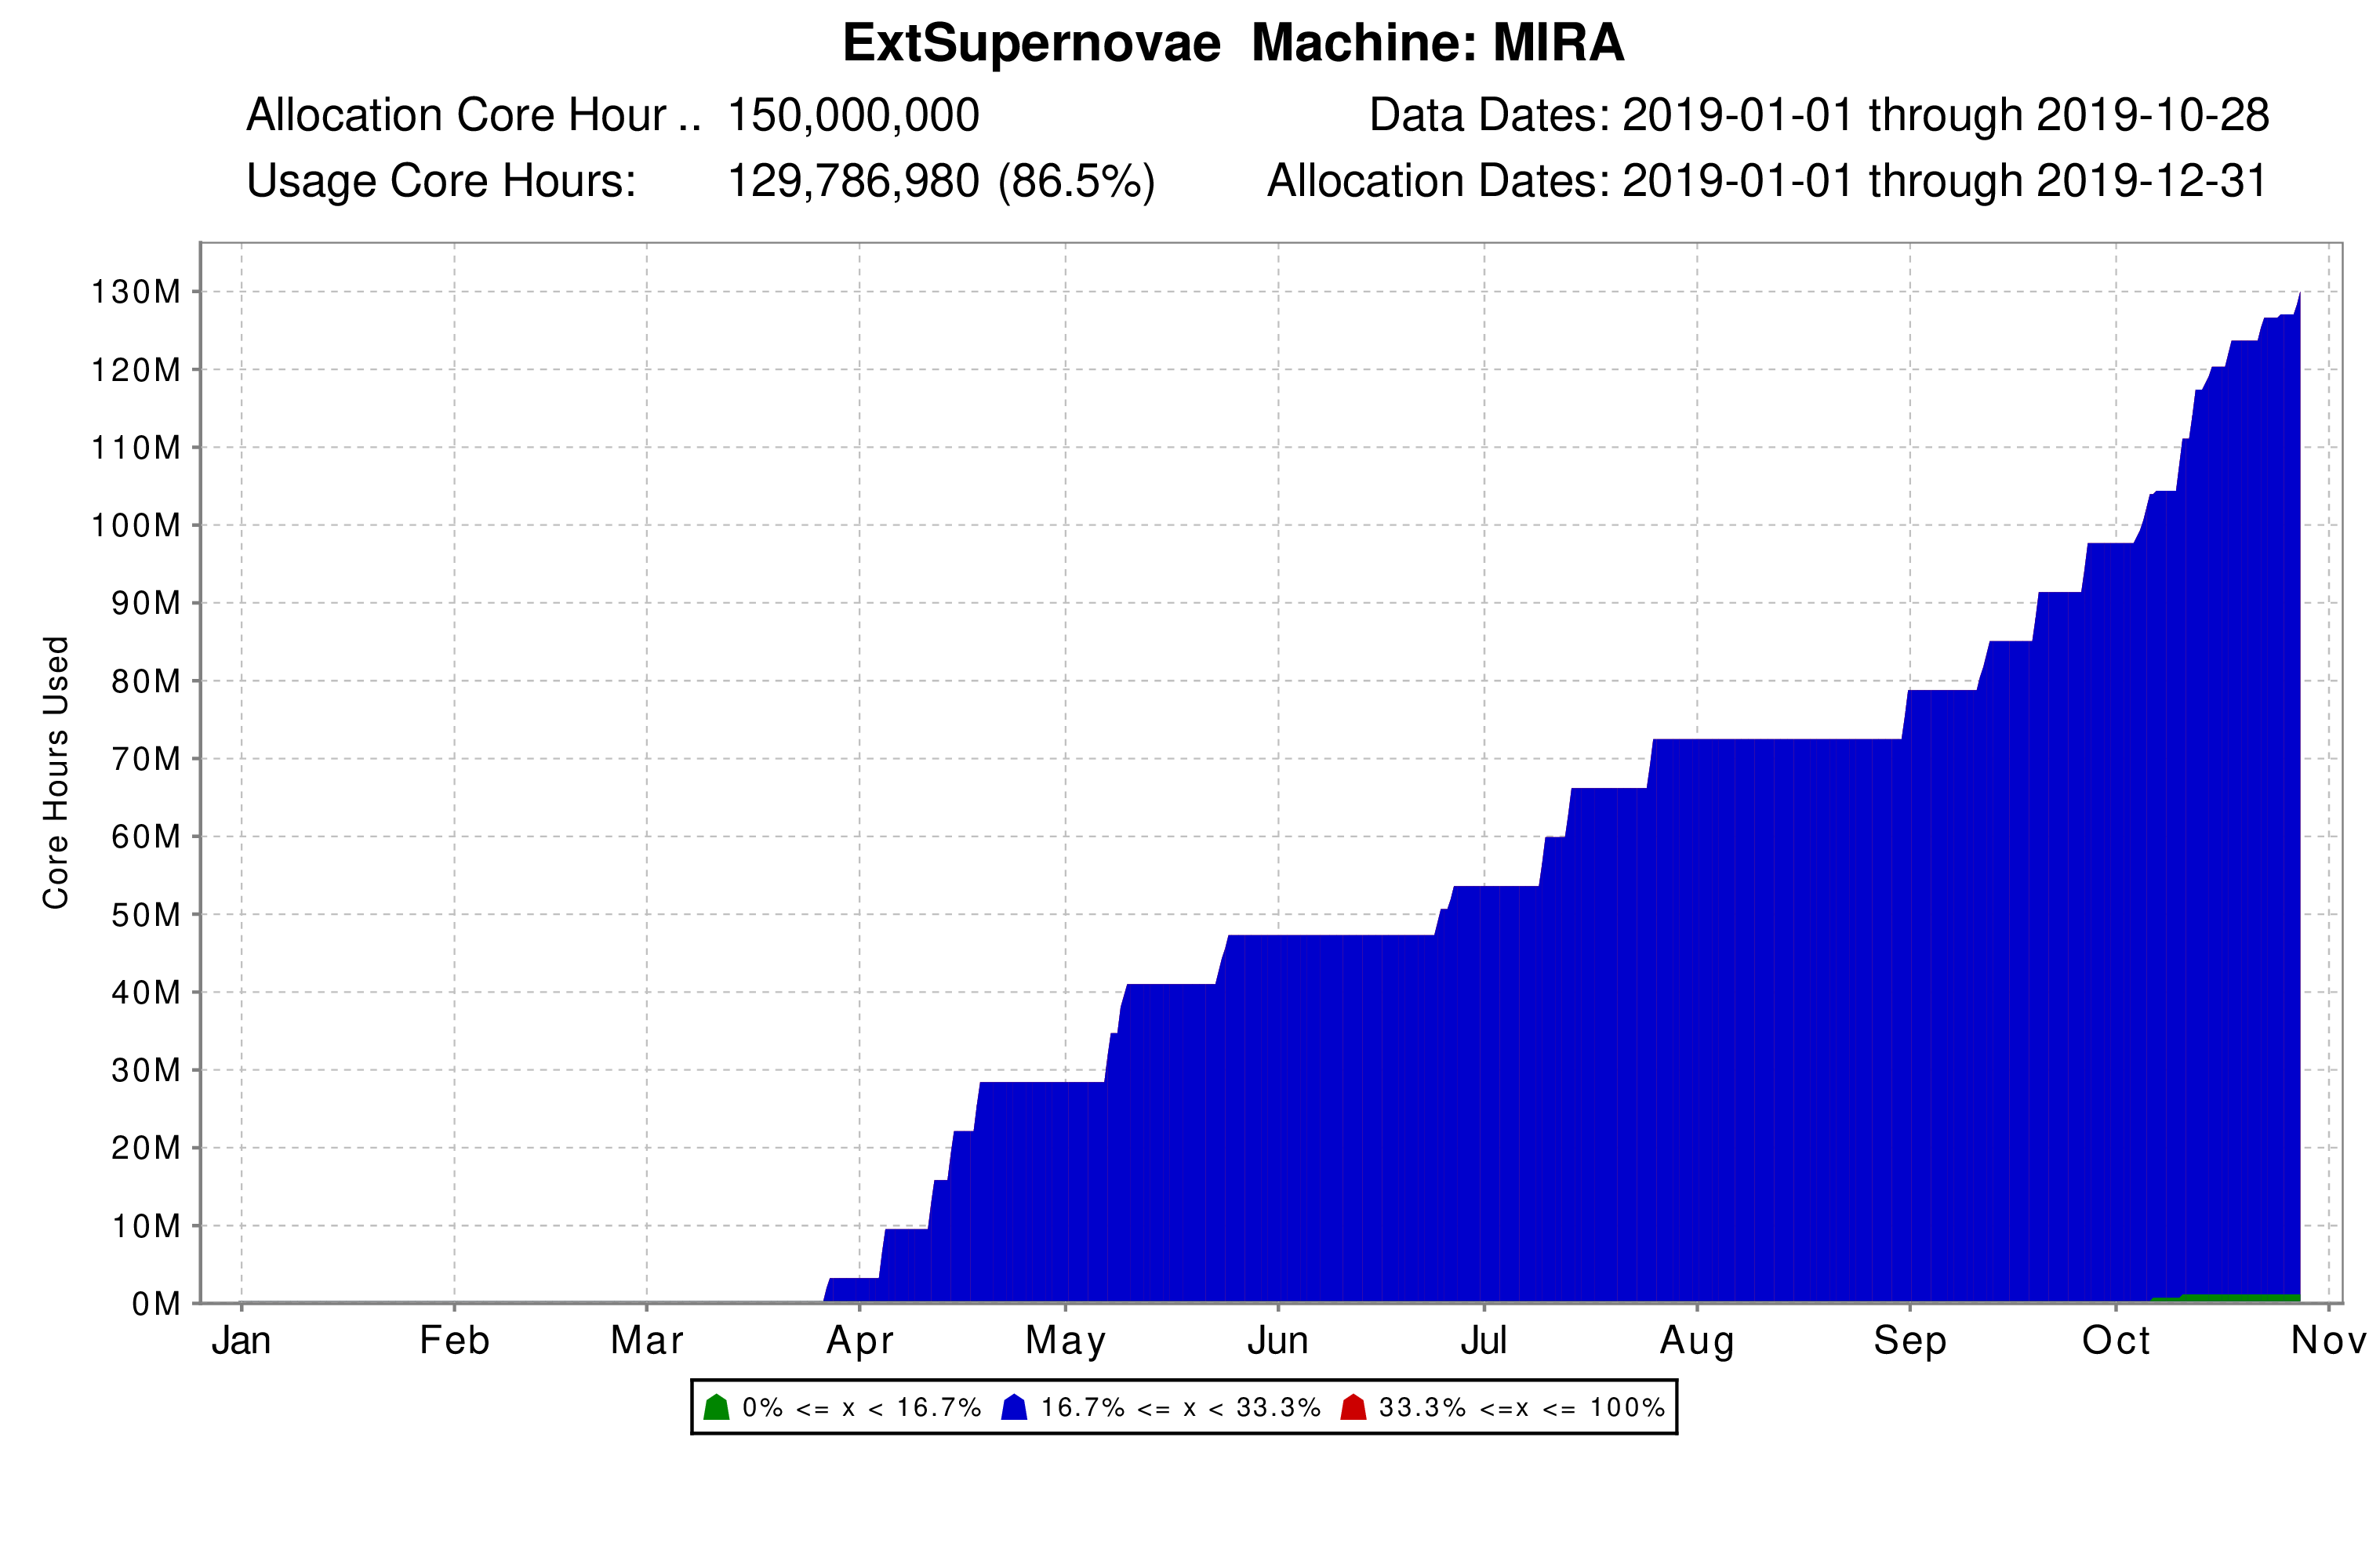
\includegraphics[width=3.25in]{categorized_hours_graph_mira.png} \\
%     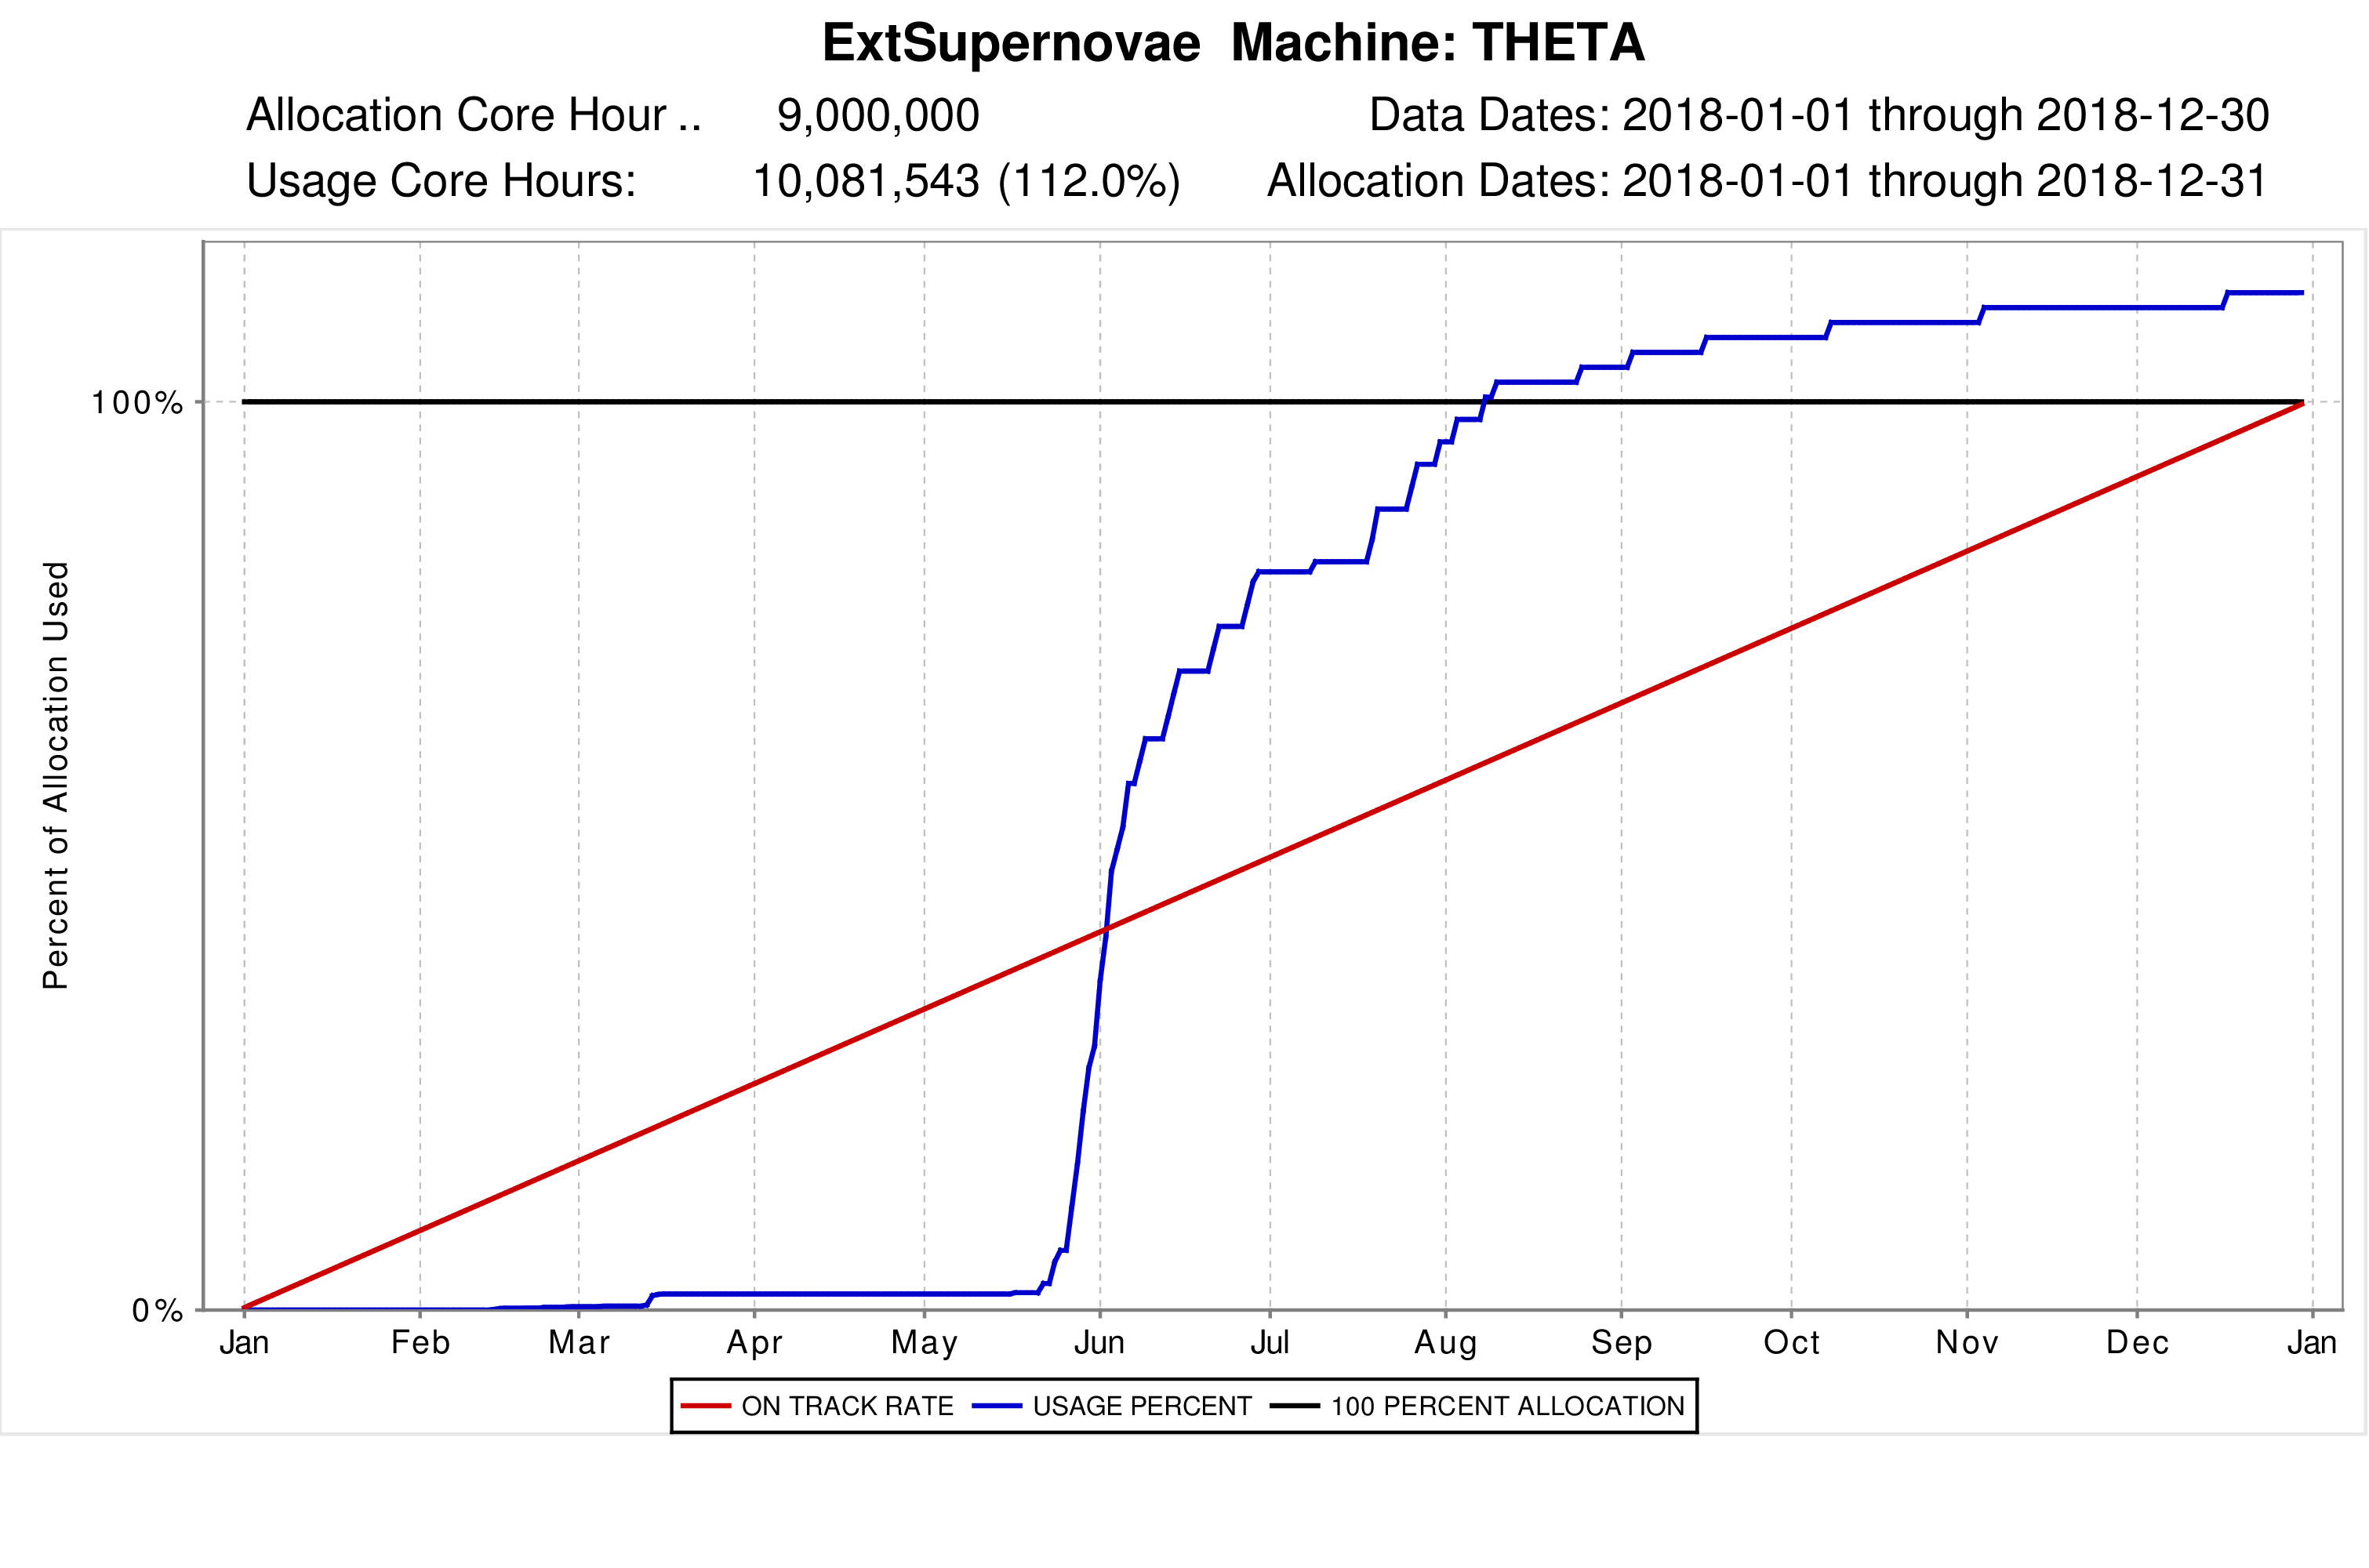
\includegraphics[width=3.25in]{on_track_graph}
%     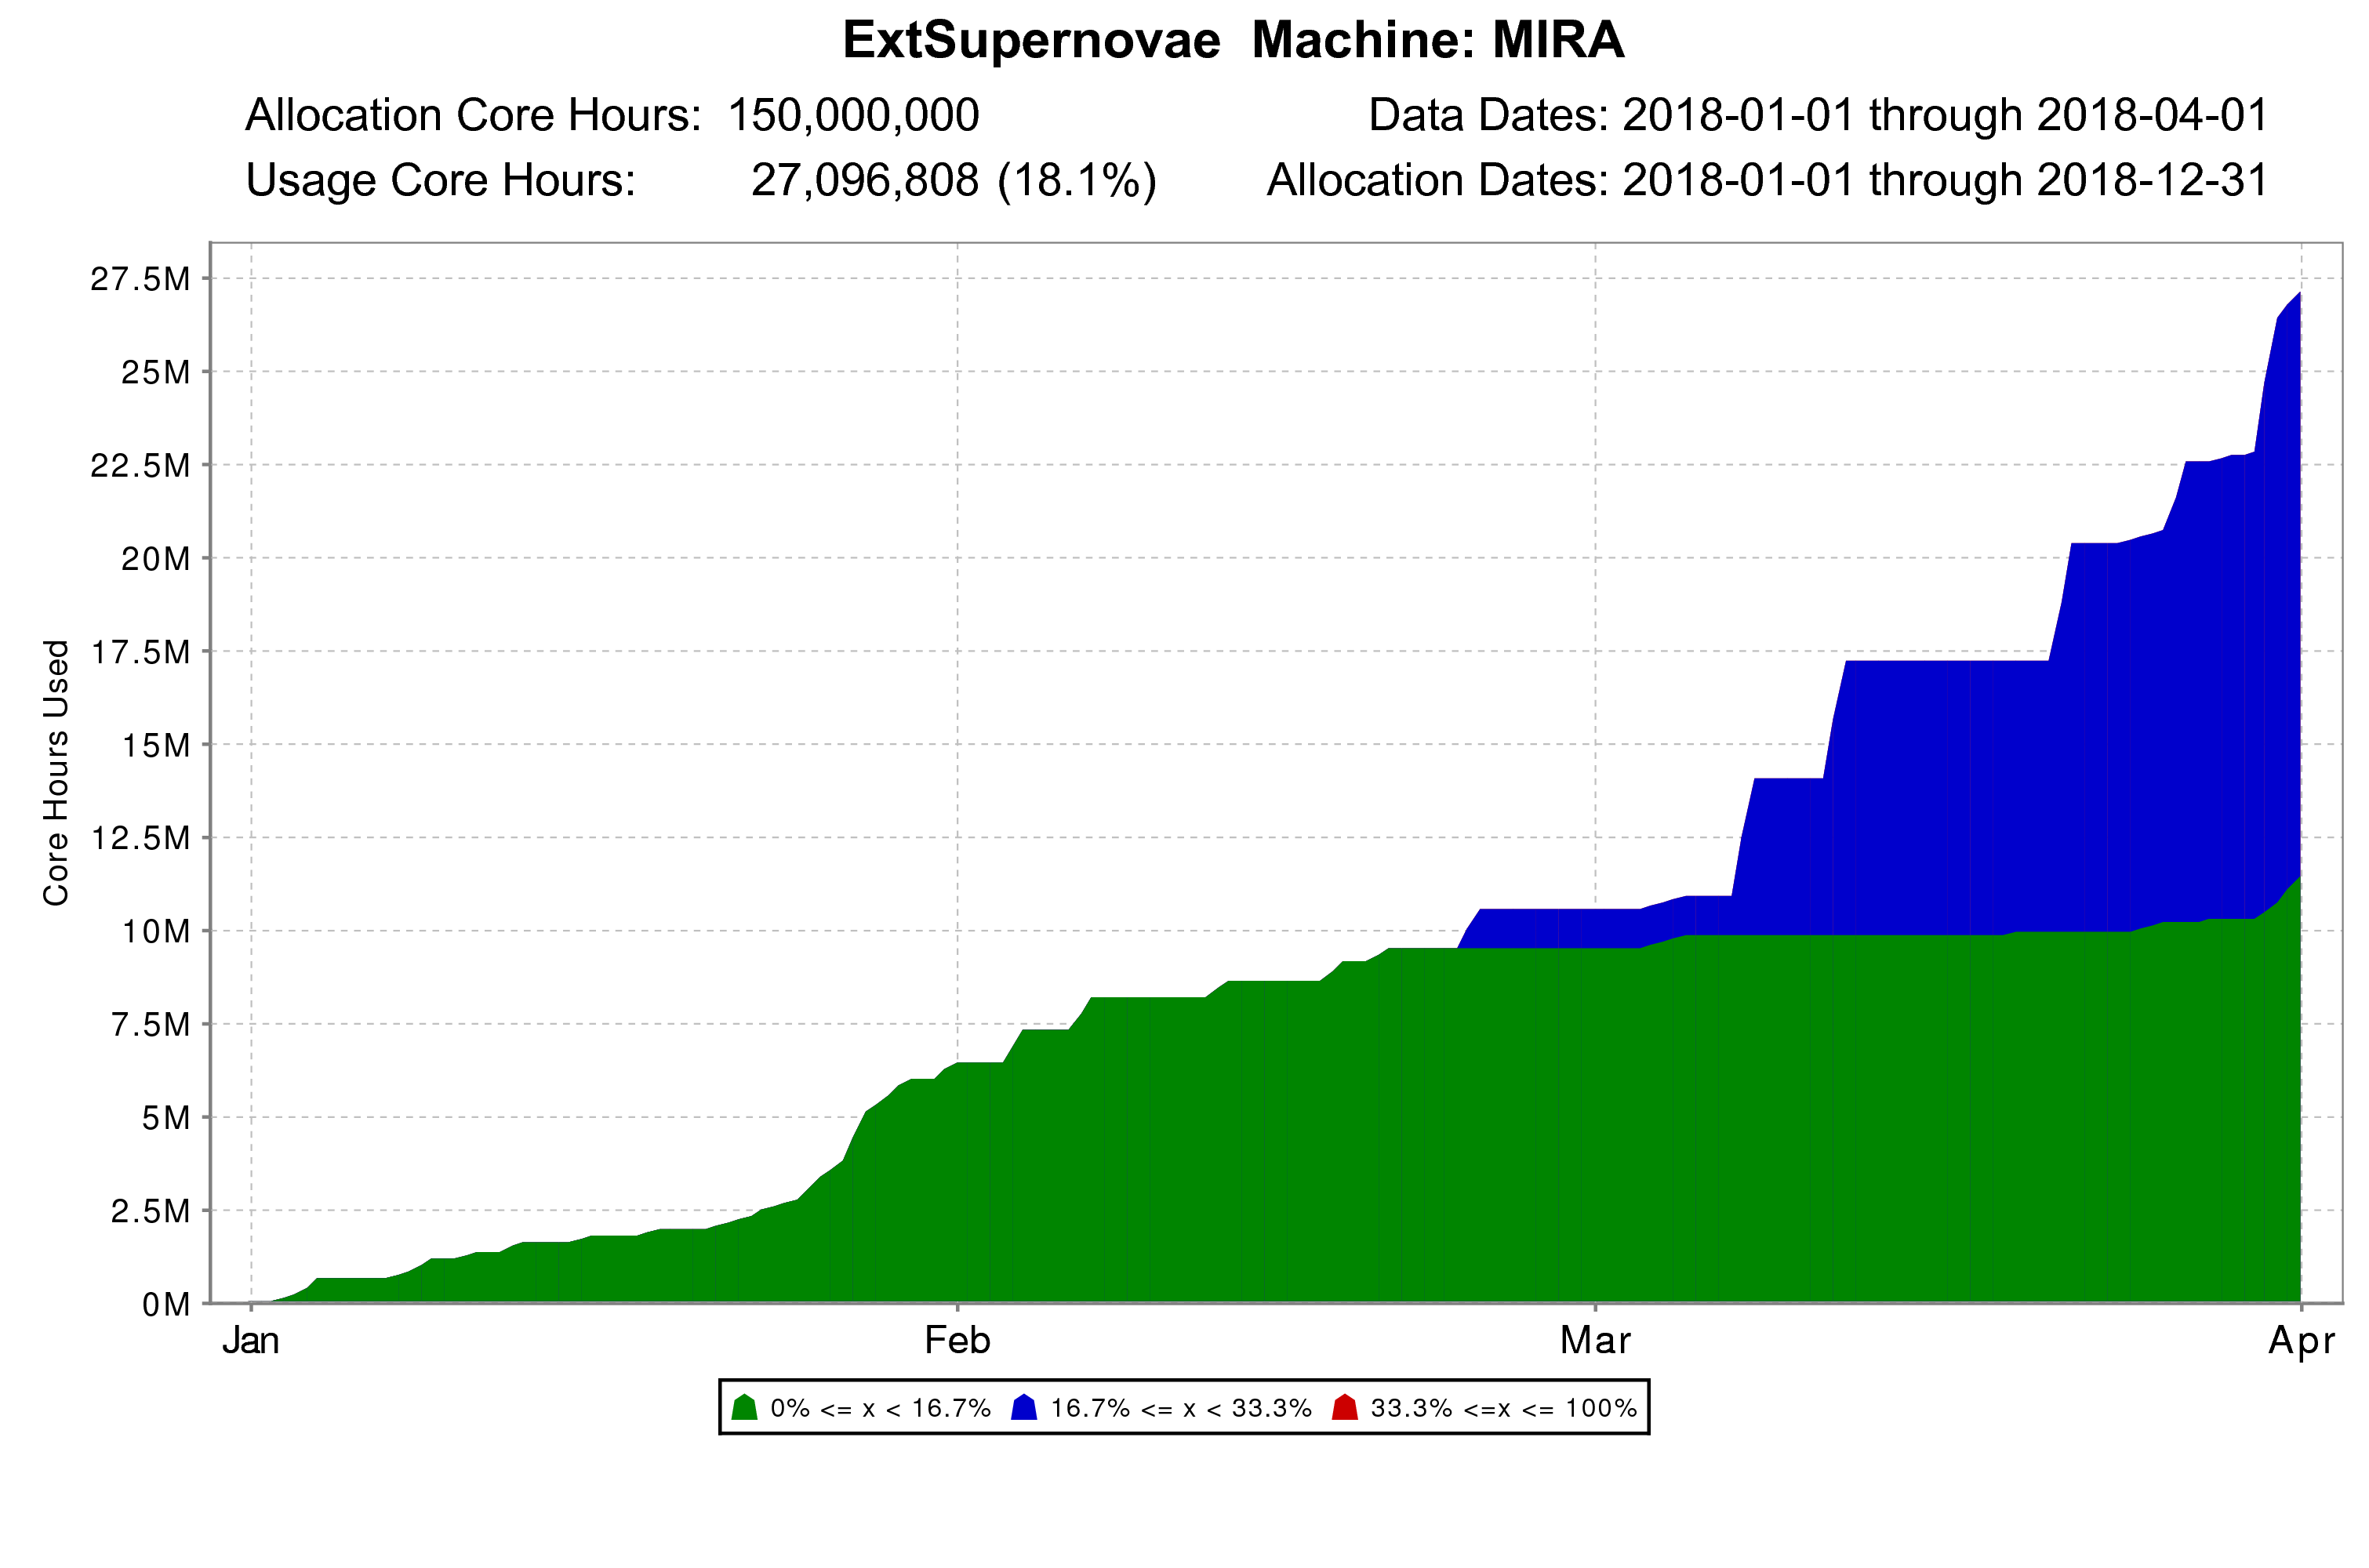
\includegraphics[width=3.25in]{categorized_hours_graph} 
%   \end{tabular}
%   \caption{Allocation usage.}
%   \label{fig:usage}
% \end{figure}

In 2019 Q1 we expended 3.2M core-hours on Mira out of our total 2019 allocation of 150M core-hours. 
This is substantially behind the linear usage curve.
During Q1 we have focussed on getting new project personnel up to speed on the project, code tuning, and implementation of new capabilities in our core-collapse supernova (CCSN) application (see below). 
We are now running one of our primary simulation milestones in the Capability queue and will start a second Capability-scale simulation in the next week or two. Unlike in years past, when our simulations started small and grew to the Capability queue, we are starting 2019 already at that scale. 
Based on past usage experience, we do not anticipate any issues returning to the ``ideal'' usage rate. 

%%%%%%%%%%%%%%%%%%%%%%%%%%%%%%%%%
\section{Report on Project Milestones}
%%%%%%%%%%%%%%%%%%%

Our milestones for Year 2, and corresponding progress, were:
\begin{enumerate}
    \item Long time simulations of MHD CCSNe - These simulations have been restarted from simulations carried over from 2018 and are running in the Capability queue.
    \item High-resolution simulation of MHD dynamos in the proto-neutron star - So far in Q1 we have analyzed simulations from 2018 that will serves as the initial conditions for this high-resolution simulation. We anticipate starting this simulation in the next week or two. Given the extreme resolution of this simulation, it will run in the Capability queue from the outset.
    \item MHD simulation of CCSN progenitors - These simulations will be started in Q2. We are tuning our progenitor application to make better use of OpenMP threading.
    \item CCSN simulation with 3D progenitors - The progenitor model for these simulations is now finished and ready to be used in CCSN simulations. We plan to run these simulations on Theta starting in Q2 or Q3.
    \item Implement microphysics from TEAMS SciDAC collaboration and neutrino-electron scattering (NES) - the TEAMS microphysics package is not yet ready for production simulations. We have during Q1 finished an implementation of NES and are now testing it in 1D and 2D simulations. We anticipate being able to use this new capability in our planned 2019 CCSN simulations. 
\end{enumerate}



%%%%%%%%%%%%%%%%%%%%%%%%%%%%%%%%%
\section{Project Productivity}
%%%%%%%%%%%%%%%%%%%

\subsection{Primary}

\noindent {\bf Publications}
\begin{itemize}
    \item \href{https://ui.adsabs.harvard.edu/#abs/2019arXiv190201340C/abstract}{``Simulating Turbulence-aided Neutrino-driven Core-collapse Supernova Explosions in One Dimension''}, Couch, S. M., Warren, M. L., O'Connor, E. P. 2019, {\itshape arXiv e-prints}, arXiv:1902.01340 
    \item \href{https://ui.adsabs.harvard.edu/#abs/2019arXiv190109055P/abstract}{``Features of Accretion Phase Gravitational Wave Emission from Two-dimensional Rotating Core-Collapse Supernovae''}, Pajkos, M. A., Couch, S. M., Pan, K., O'Connor, E. P. 2019, {\itshape arXiv e-prints}, arXiv:1901.09055 
\end{itemize}

\noindent {\bf Presentations}

\begin{itemize}
  \item ``Gravitational Waves from Core-collapse Supernovae,'' S.M. Couch, LIGO SN Group Seminar, March 2018
\end{itemize}

% \subsubsection{Secondary}

% \begin{itemize}
%   \item Co-I and postdoc Kuo-Chuan Pan started a tenure-track faculty position at National Tsing Hua University in Taiwan.
%   \item Co-I and postdoc MacKenzie Warren won a prestigious NSF Postdoctoral Fellowship.
% \end{itemize}

\section{Center Feedback}

Our catalyst, Adrian Pope, has been extremely helpful.
He is now helping us tune our code for Theta.


\section{Code Description and Characterization}

\texttt{FLASH} is a highly capable, fully modular, extensible,
community code that is widely used in astrophysics, cosmology, fluid
dynamics, and plasma physics, and other fields.  The capabilities of
the FLASH code include adaptive mesh refinement (AMR), several
self-gravity solvers, an advection-diffusion-reaction (ADR) flame
model, an accurate and detailed treatment of nuclear burning, and a
sophisticated two-moment neutrino transport scheme based on an
explicit hyperbolic solver.  The neutrino interactions are included
through the open-source neutrino interaction library
\texttt{NuLib}. We have enhanced the
performance of the two-moment neutrino transport scheme significantly
as well as upgraded the transport to now include full velocity and
gravitational red-shift dependence in the evolution equations.

\texttt{FLASH} is written in modern Fortran, with some utility
functions written in C, and a build system written in Python.  It
requires MPI library support, and either HDF5 or P-NetCDF for I/O.
Additional mathematical software, such as \texttt{Hypre}, may be
required to configure \texttt{FLASH} for particular simulations.

Algorithm classes used within \texttt{FLASH} include Sparse Linear
Algebra solvers, FFT, active and passive particles, structured grids,
and AMR.



\end{document}
